%!TEX encoding = UTF-8 Unicode
\chapter{Hybrid Testing Method on a Semi-actively Controlled Building Structure Equipped with Full-scale MR Dampers}
\label{chap:rthytem-mrdamper}

In this study, the verification of the hysteretic behavior of an MR damper and the quantitative evaluation of the seismic performance of a building structure installed with an MR damper are carried out experimentally using the hybrid testing method. This component should be an electronic control unit or a real engine. The interface between simulated and physical components is achieved through the direct transfer of electrical signals, without actuation devices\citep{christenson2008large}. As described in chapter~\ref{rthytem}, the hybrid testing method is a structural testing technique, in which the numerical integration of the equation of motion of a numerical substructure and the physical testing of an experimental substructure with severe non-linear characteristics are carried out simultaneously in real-time. In chapter~\ref{rthytem}, it has been performed both experimentally and analytically on the hybrid testing technique in order to overcome the difficulties in the testing of large-scale structures. This technique is especially useful for evaluating the performance of the nonlinear control device itself as well as that of the integrated system incorporated with the nonlinear control device such as MR damper.

\section{Outline of Methodology}
Figure~\ref{fig:8-1} shows the concept of the hybrid testing method, which is experimentally implemented in this study. As shown in Figure~\ref{fig:8-1a}, the structural response of a building model with $n$-degrees-of-freedom subjected to base input motion, $\ddot{x}_{g}(t)$, is controlled by an MR damper, which is typically located in the first story to reduce the maximum shear force of a bare structure. The whole system is divided into experimental and numerical substructures (Figure~\ref{fig:8-1b}). The MR damper is used as an experimental substructure because it is very difficult to numerically predict its exact dynamic behavior under seismic load, due to its strong non-linear characteristic of the dependency of the damper force on the loading rate and amplitude. The remaining parts, that is, the structure without an MR damper, are analytically calculated. As shown in Figure~\ref{fig:8-1c}, three procedures including the measurement of force, the numerical calculation of analytical parts, and the loading of the experimental substructure are used to implement the hybrid testing method for the whole structural control system\citep{blakeborough2001development}. First, the force acting at the interface between experimental and numerical substructures (here, the control force generated by the MR damper), is measured by the load cell attached to an actuator. The value of this measured control force is then returned to the control computer for use in the calculation of the displacement constraint condition, which should be satisfied by both the experimental and numerical substructures. Finally, the MR damper physically tested in the laboratory is loaded by an actuator with respect to the displacement response of the story installed with the MR damper. The numerical substructure surrounded by the dotted line in Figure~\ref{fig:8-1c} is calculated based on the equation of motion for the building model equipped with an MR damper that is subjected to ground input acceleration, which is represented by:

\begin{equation}\label{eq:8-1}
\matr{M}\matr{\ddot{x}}(t)+\matr{C}\matr{\dot{x}}(t)+\matr{K}\matr{x}(t) = -\matr{M}\matr{\Gamma}\ddot{x}_{g}(t)+\matr{H}f_{e}(t)
\end{equation}

where, $\matr{M}$, $\matr{C}$, and $\matr{K}$ represent the $n \times n$ structural mass, damping, and stiffness matrices, respectively; $\matr{x}(t)$ the $n\times 1$ vector of the relative structural displacement to the ground input motion; $\matr{\Gamma}$ the $n\times1$ vector of the ground input motion influence coefficients; $\matr{H}$ the $n \times 1$ vector that represents the location of the MR dampers; $\ddot{x}_{g}(t)$ the ground input acceleration; and $f_{e}(t)$ the control force exerted by the MR damper on the structure, in which subscript `$e$' represent `\textit{experimentally}' measured control force.

\begin{figure}[!ht]
\centering
\subfigure[structural control system]{
   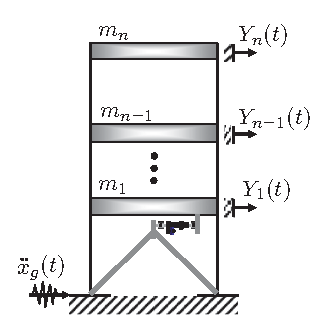
\includegraphics[width=0.3\textwidth] {figure/8-1a.eps}
   \label{fig:8-1a}\hfill
 }
\subfigure[experimental and numerical substructures]{
   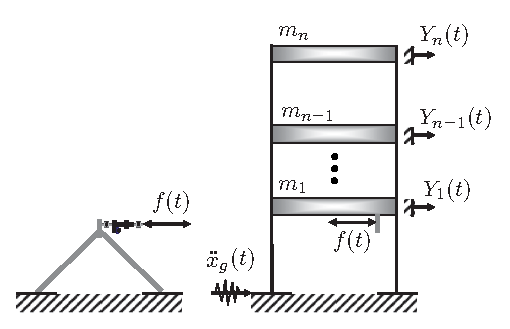
\includegraphics[width=0.5\textwidth] {figure/8-1b.eps}
   \label{fig:8-1b}
}
\subfigure[implementation of hybrid testing method]{
   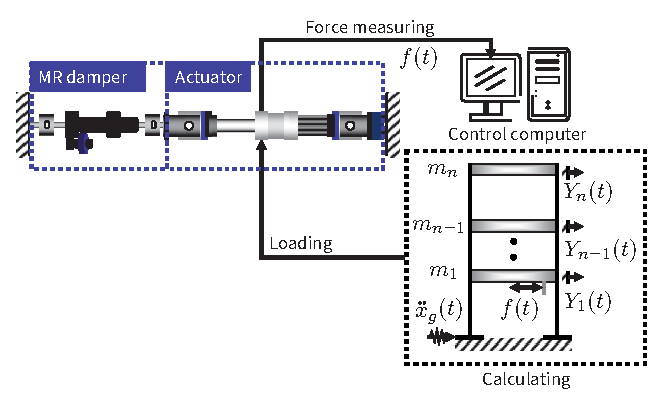
\includegraphics[width=0.8\textwidth] {figure/8-1c.eps}
   \label{fig:8-1c}
}
\caption{Conceptual view of hybrid testing method for a building with an MR damper.}
\label{fig:8-1}
\end{figure}

To perform the hybrid testing method, Eq.~\eqref{eq:8-1} is transformed into its state-space representation, which positively specifies the relationship between the input and output of the numerical substructure and can be written as:

\begin{equation}\label{eq:8-2}
\begin{aligned}
\matr{\dot{z}}_{s}(t) &= \matr{A}_{s}\matr{z}(t) + \matr{B}_{s}\matr{u}(t)\\
\matr{Y}_{s}(t) &=\matr{C}_{s}\matr{z}(t) + \matr{D}_{s}\matr{u}(t)
\end{aligned}
\end{equation}

where $\matr{z}_{s}(t) = \left\{\matr{x}(t), \matr{\dot{x}}\right\}^{\top}$ is the $2n \times 1$ system state vector; $\matr{U}(t) = \left\{f_{e}(t),\ddot{x}_{g}(t)\right\}^{\top}$ the $2\times1$ system input vector; and $\matr{Y}_{s}(t)=\matr{x}(t)$ the $n\times1$ system output vecor. The $2n\times2n$ system state matrix, $\matr{A}_{s}$, and the $2n\times2$ locaation matrix of system input, $\matr{B}_{s}$, both associated with the system state variables, are represented by:

\begin{equation}\label{eq:8-3}
\begin{aligned}
\matr{A}_{s} &= \begin{bmatrix} \matr{0}_{n\times n} & \matr{I} \\ -\matr{M}^{-1}\matr{K} & -\matr{M}^{-1}\matr{C}\end{bmatrix} \\
\matr{B}_{s} &= \begin{bmatrix} \matr{0}_{n\times1} & \matr{0}_{n\times1} \\ -\matr{M}^{-1}\matr{H} & -\matr{\Gamma} \end{bmatrix}
\end{aligned}
\end{equation}

and the $n\times n$ system out matrix, $\matr{C}_{s}$, and the $n\times2$ direct transmission matrix, $\matr{D}_{s}$, both related to the system output variables, are given by:

\begin{equation}\label{eq:8-4}
\matr{C}_{s} = \matr{I}, \matr{D}_{s} = \matr{0}_{n\times1}
\end{equation}

In Eqs.~\eqref{eq:8-3} and \eqref{eq:8-4}, $\matr{I}$ is the $n\times n$ unit matrix, while $\matr{0}_{n\times n}$ and $\matr{0}_{n\times1}$ are the $n\times n$ and $n\times1$ zero matrices, respectively. Note that, in the actual implementation of hybrid testing method, the system output vector, $\matr{Y}_{s}(t)$, in Eq.~\eqref{eq:8-2} should be designated as the story drifts where the MR dampers are installed and Eq.~\eqref{eq:8-4} should also be modified because these story drifts affect the system output vector.

A full-scale five-story steel frame building is considered as the model of the numerical substructure to use in the structural modal testing of this study, as shown in Figure~\ref{fig:7-2}. 

\begin{figure}[ht]
\centering
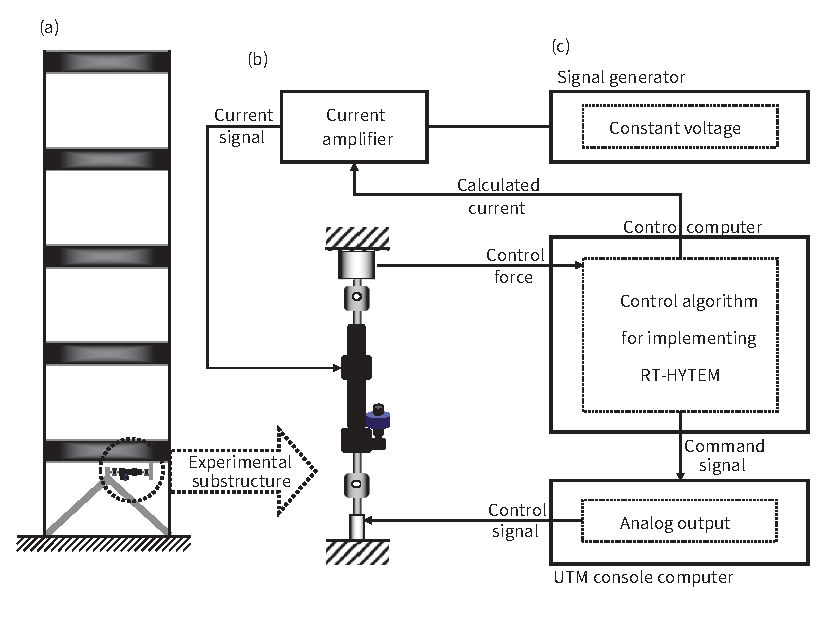
\includegraphics[width=1\textwidth] {figure/8-3.eps}
\caption{Schematic view of experimental set-up: (a) building model installed with an MR damper, (b) UTM installed MR damper, and (c) experimental instrumentation.}
\label{fig:8-3}
\end{figure}


When these identified structural properties are incorporated in the numerical substructure, Eqs.~\eqref{eq:8-2}, \eqref{eq:8-3} and \eqref{eq:8-4} can be rewritten as Eqs.~\eqref{eq:8-8}, \eqref{eq:8-9} and \eqref{eq:8-10}, respectively.

\begin{equation}\label{eq:8-8}
\begin{aligned}
\matr{\dot{z}}_{n}(t) & = \matr{A}_{n}\matr{z}_{n}(t) + \matr{B}_{n}\matr{u}(t) \\
\matr{Y}_{n}(t) & = \matr{C}_{n}\matr{z}_{n}(t) + \matr{D}_{n}\matr{u}(t)
\end{aligned}
\end{equation}

where, $\matr{Z}_{n}(t) = \left\{ x_{1}(t),...,x_{5}(t),\dot{x}_{1}(t),...,\dot{x}_{5}(t)\right\}^{\top}$ is the $10\times1$ system state vector; $\matr{u}(t)=\left\{f_{e}(t), \ddot{x}_{g}(t)\right\}^{\top}$ the $2\times1$ system input vector; and $\matr{Y}_{n}(t) = \left\{x_{1}(t),...,x_{5}(t),\dot{x}_{1}(t),...,\dot{x}_{5}(t),\ddot{x}_{1}(t),...,\ddot{x}_{5}(t)\right\}^{\top}$ the $15\times1$ system output vector. The $10\times10$ system state matrix, $\matr{A}_{n}$, and the $10\times2$ location matrix of system input, $\matr{B}_{n}$, are represented by Eq.~\eqref{eq:8-9}:

\begin{equation}\label{eq:8-9}
\begin{aligned}
\matr{A}_{n} & = \begin{bmatrix} \matr{0}_{5\times5} & \matr{I} \\ -\matr{M}_{5}^{-1}\matr{K}_{5} & -\matr{M}_{5}^{-1}\matr{C}_{5}\end{bmatrix} \\
\matr{B}_{n} & = \begin{bmatrix} \matr{0}_{5\times1} & \matr{0}_{5\times1} \\ -\matr{M}_{5}^{-1}\matr{H}_{5} & -\matr{\Gamma}_{5} \end{bmatrix}
\end{aligned}
\end{equation}

and the $15\times10$ system out matrix, $\matr{C}_{5}$, and the $15\times2$ direct transmission matrix, $\matr{D}_{5}$ are given by Eq.~\eqref{eq:8-10}

\begin{equation}\label{eq:8-10}
\begin{aligned}
\matr{C}_{n} & = \begin{bmatrix} \matr{I} & \matr{0}_{5\times5} \\ \matr{0}_{5\times5} & \matr{I} \\ -\matr{M}_{5}^{-1}\matr{K}_{5} & -\matr{M}_{5}^{-1}\matr{C}_{5}\end{bmatrix} \\
\matr{D}_{n} & = \begin{bmatrix} \matr{0}_{5\times1} & \matr{0}_{5\times1} \\ \matr{0}_{5\times1} & \matr{0}_{5\times1} \\ -\matr{M}_{5}^{-1}\matr{H}_{5} & -\matr{\Gamma}_{5} \end{bmatrix}
\end{aligned}
\end{equation}

In Eq.~\eqref{eq:8-9} and \eqref{eq:8-10}, $\matr{I}$ is the $5\times5$ unit matrix, while $\matr{0}_{5\times5}$ and $\matr{0}_{5\times1}$ are the $5\times5$ and $5\times1$ zero matrices, respectively.

\section{Controller Design Strategy for the Hybrid Testing Method}
\subsection{Experimental Set-up}
In general, the successful experimental implementation of the hybrid testing method with high accuracy depends strongly on the dynamic performance of the actuators used to excite the experimental substructure in the test. Namely, the actuators used in the test should promptly react to applied command signals and load the experimental substructure. In this study, a universal testing machine (UTM), which is commonly used for the performance test of various structural materials, is utilized as an actuator to load the experimental part. Figure~\ref{fig:8-2} shows the experimental set-up using UTM with the maximum loading capacity of 200kN and excitation frequency range of 0-10 Hz (Model name STL-HU10T). An MR damper, which can develop a control force ranging from 3 to 12 kN, is connected to this system. As shown in Figure~\ref{fig:8-3}, in order to perform the hybrid testing method, three apparatuses with interconnected functions are equipped with the experimental set-up. The main task of the signal generator is to generate the current signal, by which an MR damper is operated, and control force is exerted on the UTM. The control computer with a digital signal processing (DSP) board calculates the responses of the numerical substructure using the input (the control force measured from a load cell of the UTM) and sends the command signal to the UTM console computer. The primary task of the UTM console computer is to transfer the command signal generated by the control computer, according to the control algorithm for implementing the hybrid testing method, to the UTM. Finally, the UTM excites the experimental part according to this control signal.

\begin{figure}[!ht]
\centering
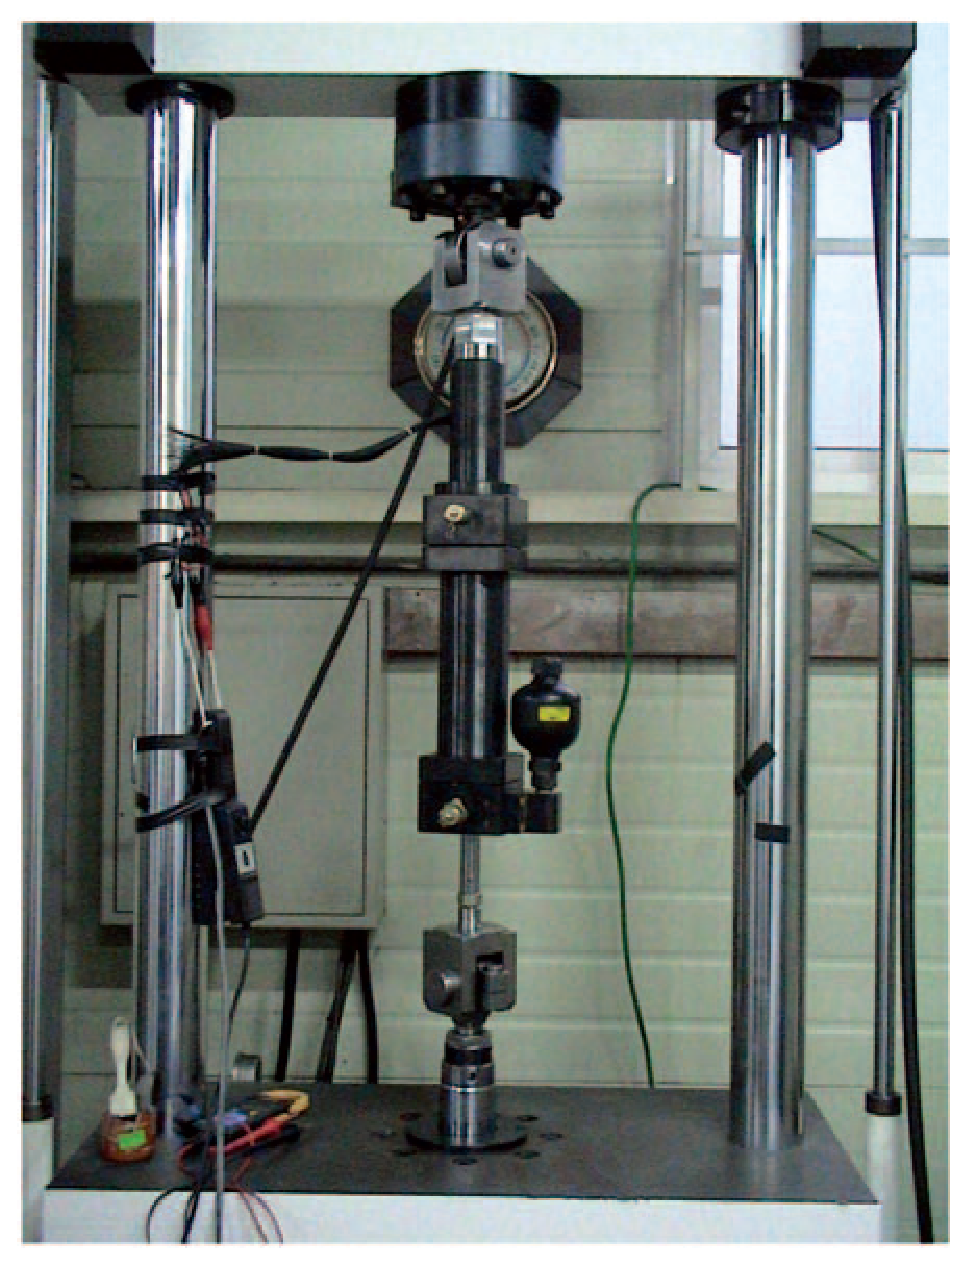
\includegraphics[width=0.8\textwidth] {figure/8-2.eps}
\caption{Configuration of experimental system.}
\label{fig:8-2}
\end{figure}


\subsection{Controller Design of UTM}
In order to accurately load the experimental substructure by an actuator and in accordance with the control algorithm of the hybrid testing method, the dynamic property of the actuator itself between the command signal and the measured response should be appropriately compensated. Without this compensation, problems can occur with the experimental results such as chattering problems or the operating performance of the testing system can be degraded. In particular, during structural testing associated with vibration control issues, the control force often acts as an external load, and as a result, the experimental system can become unstable.

In order to experimentally measure the dynamics of UTM, white noise with a frequency ranging from 0 to 10Hz is used as the command signal, as shown in Figure~\ref{fig:8-3} and the corresponding displacement of UTM that is driven by this signal are then measured. Using these input and output data sets in the time domain, the transfer function in the frequency domain, which corresponds to the dynamics of the UTM itself, is obtained.

The phase delay is compensated using the inverse transfer function (ITRF; \citet{lee2007real,lee2007realb}), in which the relationship between the input and output in the transfer function is reversed. Accordingly, the measured ITRF is obtained with the input of the measured displacement of the UTM and the output of the command signal, as shown by the dotted lines in Figure~\ref{fig:8-6}. This measured ITRF should be incorporated in the control computer as part of the control algorithm shown in Figure~\ref{fig:8-3}, in order to compensate the phase delay of the UTM and to correctly excite the experimental substructure. The measured ITRF is approximated using the \code{invfreqs} command in MATLAB\citep{coleman1999optimization}, which finds the real numerator and denominator coefficient vectors of the approximated transfer function in the form of a fractional expression by adopting the damped Gauss-Newton method for iterative search, which minimizes the sum of the squared error between the measured and the approximated frequency response points\citep{dennis1983numerical}. The approximation result is shown by the solid line in Figure~\ref{fig:8-6} is given by the following second-order linear analog filter.

\begin{equation}\label{eq:8-11}
G^{-1}(s) = \frac{7.1945s^2 + 636.4862s + 27368.6533}{s^2 + 412.4726s + 27758.6756}
\end{equation}

where the Laplace variable, $s$, equals $j\omega$ with the imaginary constant, $j$.

Figure~\ref{fig:8-6} shows that, at 5 Hz, compensation on phase lag is attained only by 20$\circ$ with the approximated ITRF, while the phase lag of 60$\circ$ is observed in the measured ITRF. Further compensation would be possible with the use of other filters. However, further compensation is excluded here since it would have resulted in an unstable ITRF.

\begin{figure}[H]
\centering
\subfigure[Magnitude]{
   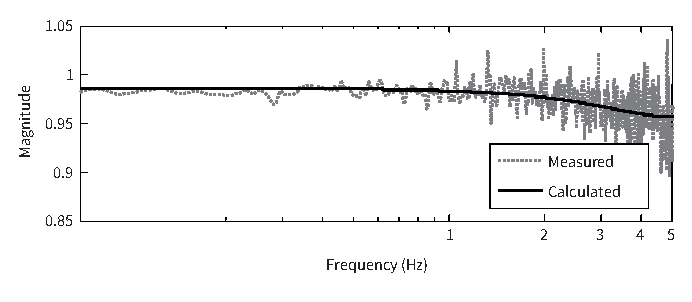
\includegraphics[width=0.6\textwidth] {figure/8-6a.eps}
   \label{fig:8-6a}\hfill
}
\subfigure[Phase]{
   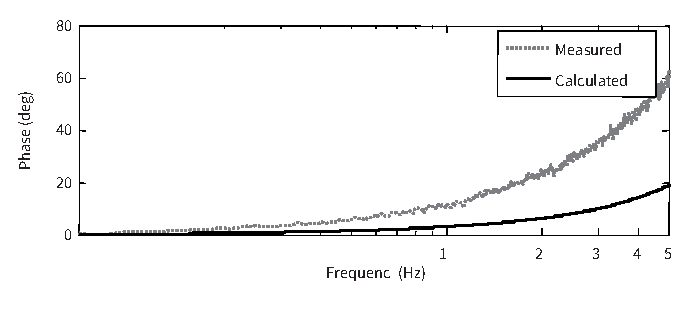
\includegraphics[width=0.6\textwidth] {figure/8-6b.eps}
   \label{fig:8-6b}
}
\caption{Measured and approximated ITRFs from the displacement of UTM to the command signal.}
\label{fig:8-6}
\end{figure}

Eq.\eqref{eq:8-11} is converted into the following statespace realization for implementation in the control computer.

\begin{equation}\label{eq:8-12}
\begin{aligned}
\matr{y}_{s} & = \matr{A}_{i}\matr{y}_{s}(t) + \matr{B}_{i}r(t) \\
c(t) &= \matr{C}_{i}\matr{y}_{s}(t) + D_{i}r(t)
\end{aligned}
\end{equation}

where $\matr{y}_{s}$, $r(t)$ and $c(t)$ are the $2\times1$ state vector, the $1\times1$ reference signal, and the $1\times1$ command signal of the UTM, respectively; and $\matr{A}_{i}$, $\matr{B}_{i}$, $\matr{C}_{i}$ and $\matr{D}_{i}$ are the $2\times2$, $2\times1$, $1\times2$ and $1\times1$ system matrices, respectively.

\section{Experimental verification}
\subsection{Integrated Controller of the Numerical Substructure and UTM}

The numerical substructure and the approximated ITRF explained above are incorporated into the control computer as an integrated controller to implement the hybrid testing method, as shown by the shaded area in Figure~\ref{fig:8-7}. First, when the constant current sent from the signal generator for the passive control test and the calculated current of semi-active control algorithms sent from the analog output for the semi-active control test are applied to the MR damper, the control force proportional to the magnitude of the current signal is developed and transferred to the UTM. The drift response, $x_{1}(t)$, of the first story where the MR damper is positioned, is then calculated from the numerical substructure, given by Eq.~\eqref{eq:8-8}, with two inputs: the control force, $f_{e}(t)$, measured from the load cell attached to the UTM and the ground input acceleration, $\ddot{x}_{g}(t)$ given by the user. The motion of the UTM is driven by the controller using the ITRF, represented by Eq~\eqref{eq:8-12} so that the UTM itself operates as the first story where the MR damper is located and excites the MR damper that should be physically tested. In the actual experimental implementation of hybrid testing method, the continuous filters shown in Figure~\ref{fig:8-7} are converted into discrete filters with a time interval of 0.01s, while MATLAB \textit{Simulink}\citep{simulink2009version} and \textit{Real-Time Windows Target}\citep{targetuser} are used as the control system.

\subsection{Experimental Verification for Simple Bouc-Wen Model}

The hybrid testing method with a sinusoidal wave excitation is carried out to investigate the hysteretic behavior of the MR damper and to verify the hybrid testing method experimentally implemented in this study. A current of 0 A is applied to the MR damper and a sine wave with a frequency of 0.52 Hz, which corresponds to the fundamental frequency of the numerical substructure, and with an amplitude of $5m/s^{2}$ is used as the ground input acceleration as shown in Figure~\ref{fig:8-7}.

\begin{figure}[H]
\centering
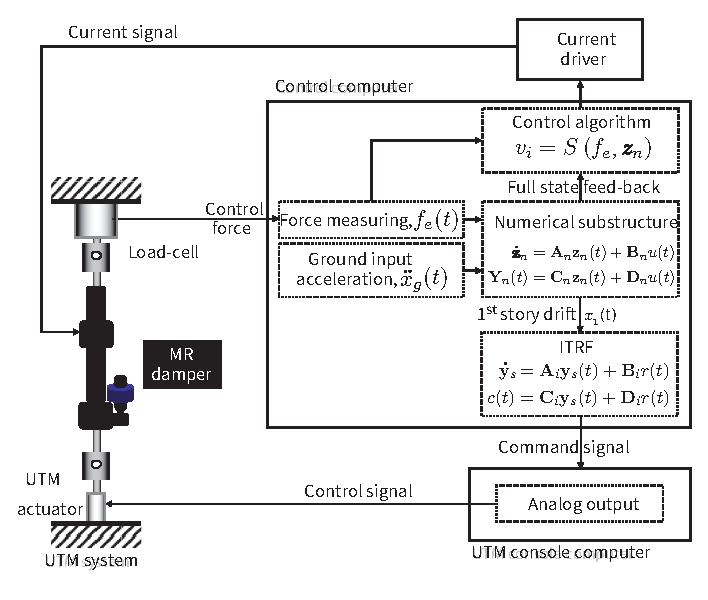
\includegraphics[width=0.8\textwidth] {figure/8-7.eps}
\caption{Integrated controller for implementing RTHTM.}
\label{fig:8-7}
\end{figure}

Parametric identification is then performed to find the numerical model of the MR damper on the basis of the experimentally measured hysteretic loop. The Bouc-Wen model is widely used for modeling various hysteretic loops\citep{wen1976method}. The control force by the MR damper can also be specified using this model. The force described by this model is represented by:

\begin{equation}\label{eq:8-13}
f_{MR}(t) = \alpha z(t) + c_{MR}\dot{x}_{1}(t) + k_{MR}x_{1}(t) + f_{0}
\end{equation}

where, $k_{MR}$ and $c_{MR}$ are the stiffness and viscosity of the MR damper; $f_{0}$ the initial friction force; $z$ a dimensionless valuable introduced to describe the hysteresis; and $\alpha$ a variable that regulates the effect of $z$ on $f_{MR}(t)$ which depends on the magnetic field; $z$ is given by the following differential equation.

\begin{equation}\label{eq:8-14}
\dot{z}(t) = -\gamma |\dot{x}_{1}(t)| z(t) |z(t)|^{n-1}-\beta\dot{x}_{1}(t)|z(t)|^{n}+A\dot{x}_{1}(t)
\end{equation}

where $\gamma$, $\beta$, $A$ and the superscript $n$ are the coefficients determining the shape of the hysteretic curve.

The eight parameters in Eqs.~\eqref{eq:8-13} and \eqref{eq:8-14} ($\alpha$, $c_{MR}$, $k_{MR}$, $f_{0}$, $\gamma$, $n$, $\beta$ and $A$) are identified using
least-squares optimization to minimize the performance index defined as:

\begin{equation}\label{eq:8-15}
J\left(\matr{p}\right) = \sum_{k=1}^{N}\left[f_{e}\left(k\cdot\Delta T \right) - f_{MR}\left(\matr{p}, k\cdot\Delta t \right)\right]^{2}
\end{equation}

where $f_{e}\left(k\cdot\Delta t\right)$ represents the force data measured at the $k-$th sampling time; $\matr{p}$ the $1\times8$ vector of the identification parameter, $\left\{ \alpha, c_{MR}, k_{MR}, f_{0}, \gamma, n, \beta, A \right\}$; and $f_{MR}\left(\matr{p},k\cdot\Delta t\right)$ the force obtained at the $k-$th calculating time from Eq.~\eqref{eq:8-13} and \eqref{eq:8-14} using the parameter $\matr{p}$.

This procedure is carried out using MATLAB subroutines\citep{coleman1999optimization}, and the identified parameters are given by:

\begin{equation}\label{eq:8-16}
\begin{aligned}
\alpha &=13288.130 (N/m), & c_{MR} = 81418.582 (N\cdot s/m), \\
k_{MR} &=16647.456 (N/m), & f_{0} = 6.10 (N), \\
n &= 3.0581, & \gamma = 471409.377 (m^{-n}),\\
\beta&=335518.804 (m^{-n}), & A=497.295
\end{aligned}
\end{equation}

A comparison between the calculated and experimental responses is provided in Figure~\ref{fig:8-8}. The displacement and velocity in Figures~\ref{fig:8-8b} and ~\ref{fig:8-8c} correspond to the first-story drift and velocity responses, respectively. The Bouc-Wen model represents the force-displacement and the force-velocity hysteretic behaviors of the damper well.

\begin{figure}[H]
\centering
\subfigure[time history of force]{
   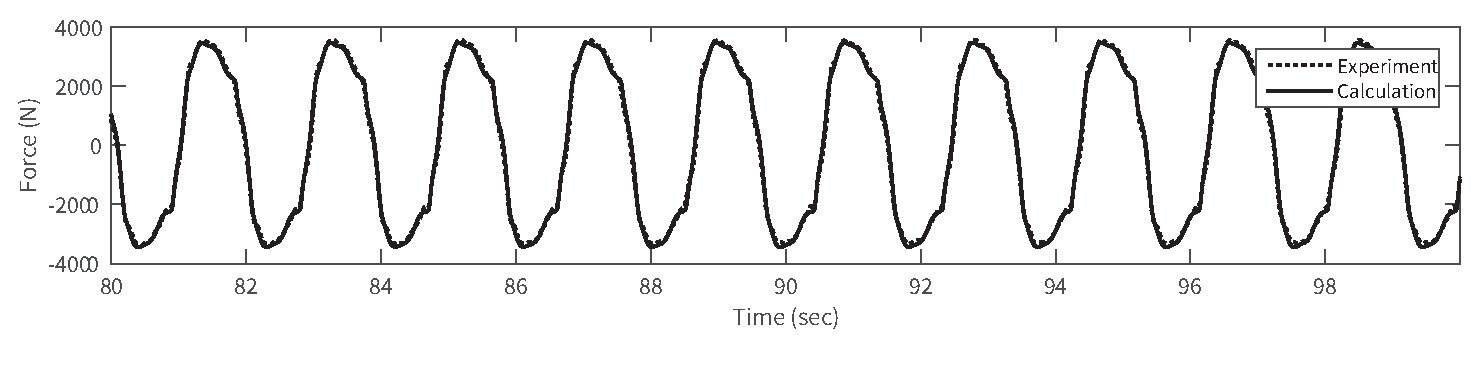
\includegraphics[width=0.9\textwidth] {figure/8-8a.eps}
   \label{fig:8-8a}
}
\subfigure[force-displacement relation]{
   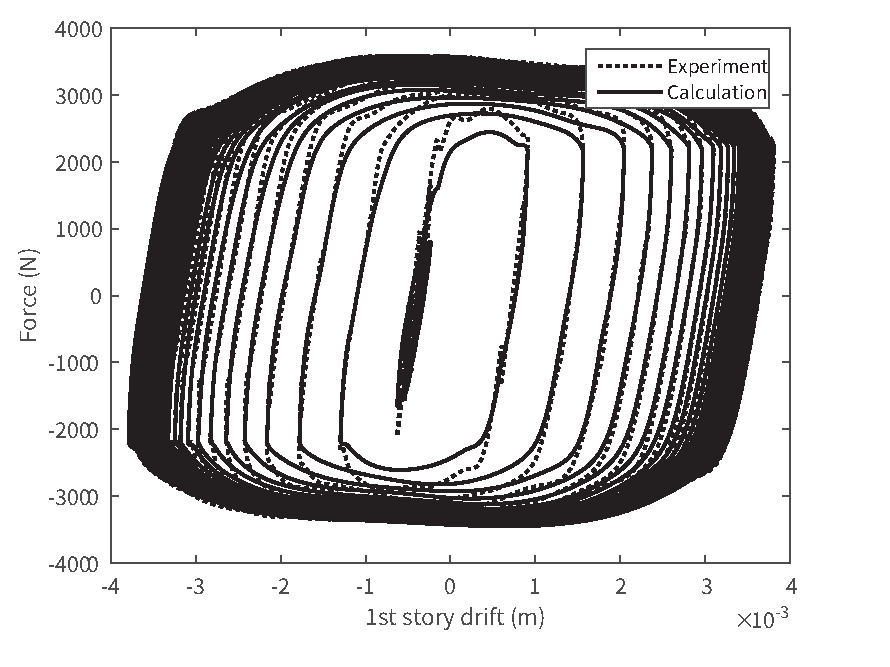
\includegraphics[width=0.45\textwidth] {figure/8-8b.eps}
   \label{fig:8-8b}
}
\subfigure[force-velocity relation]{
   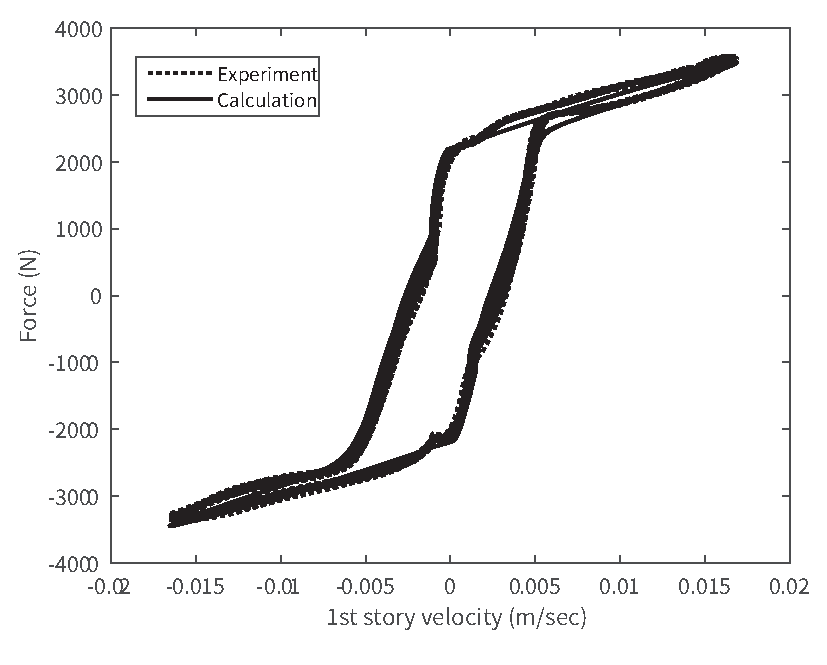
\includegraphics[width=0.42\textwidth] {figure/8-8c.eps}
   \label{fig:8-8c}
}
\caption{Comparison between calculated and experimentally measured responses for the Bouc-Wen model.}
\label{fig:8-8}
\end{figure}

The hybrid testing method implemented in this study is verified by the experiment using the excitation of historical seismic measurements. Four different records of earthquake acceleration measurements taken at El Centro, Hachinohe, Kobe, and Northridge are used as ground input acceleration in Figure~\ref{fig:8-7} by multiplying them by 0.05. Also, the current of 0 [A] is applied to an MR damper in the same manner as the sinusoidal excitation test above. In addition to the measurement of the control force produced by an MR damper, given by Eqs.~\eqref{eq:8-8}-\eqref{eq:8-10}, the structural displacement, velocity, and absolute acceleration responses are obtained from the hybrid testing method for earthquake excitations. Figures~\ref{fig:8-9} and \ref{fig:8-10} show a comparison of the responses measured by hybrid testing method, as shown in Figure~\ref{fig:8-7}, with those calculated from the five-story building model installed with an MR damper with the identified parameters such as in Eq.~\eqref{eq:8-16}, in order to compute the control force. 

\begin{figure}[H]
\centering
\subfigure[absolute acceleration responses]{
   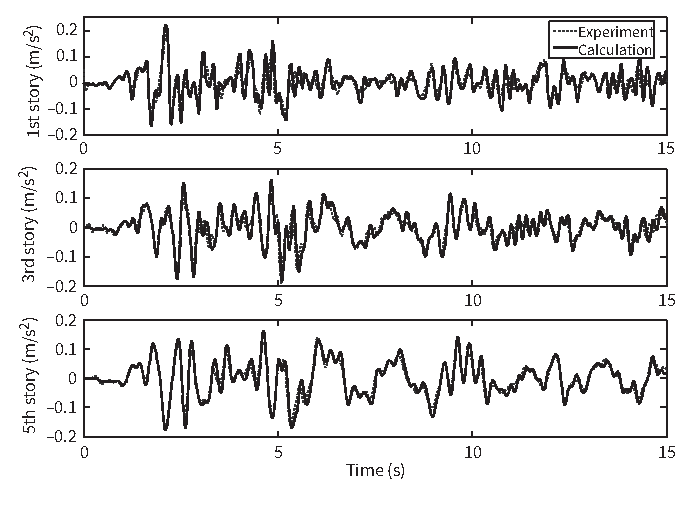
\includegraphics[width=0.8\textwidth] {figure/8-9a.eps}
   \label{fig:8-9a}
}
\subfigure[displacement responses]{
   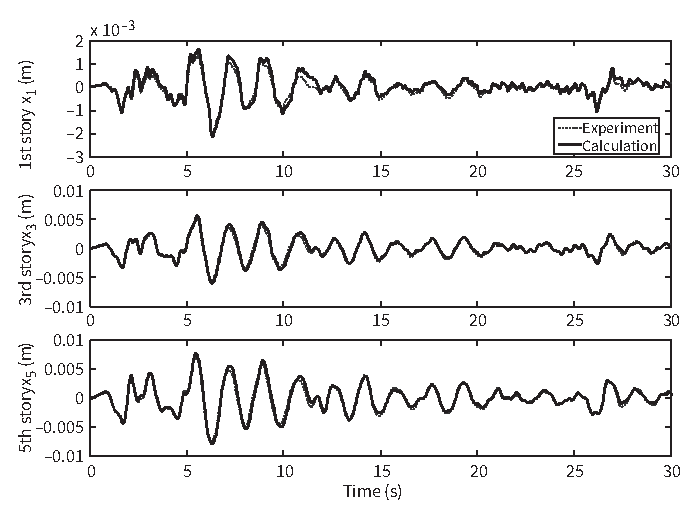
\includegraphics[width=0.8\textwidth] {figure/8-9b.eps}
   \label{fig:8-9b}
}
\caption{Comparison between calculated and experimentally measured responses under El Centro earthquake excitation.}
\label{fig:8-9}
\end{figure}

In addition, the measured and calculated hysteretic behaviors, shown in Figures~\ref{fig:8-11} and \ref{fig:8-12}, are compared for different seismic excitations. Figures~\ref{fig:8-9} and \ref{fig:8-10} show that the two results agree well with each other. Figures~\ref{fig:8-11} and \ref{fig:8-12} show that the Bouc-Wen model successfully predicted the overall hysteretic behaviors. In particular, the Bouc-Wen model successfully predicted the hysteretic behavior of an MR damper under the excitation of the seismic measurements of a narrow frequency band, such as those of the Kobe and Northridge earthquakes corresponding to the representative examples of near-fault source ground motion.

\begin{figure}[H]
\centering
\subfigure[absolute acceleration responses]{
   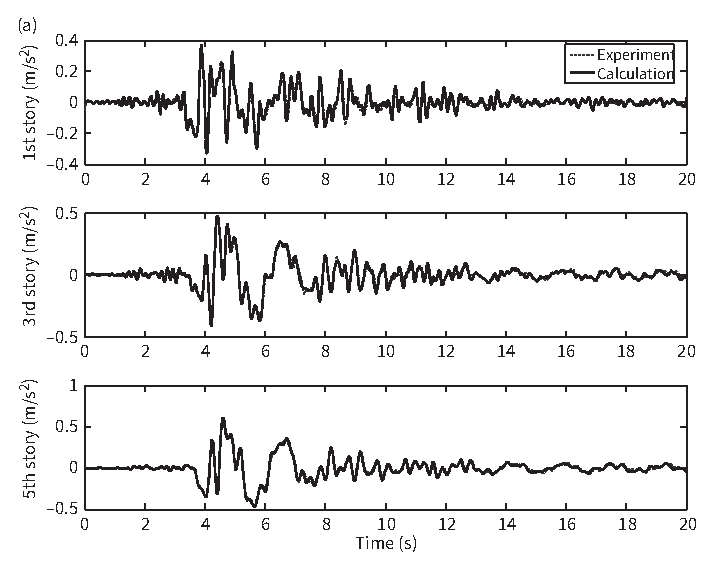
\includegraphics[width=0.8\textwidth] {figure/8-10a.eps}
   \label{fig:8-10a}
}
\subfigure[displacement responses]{
   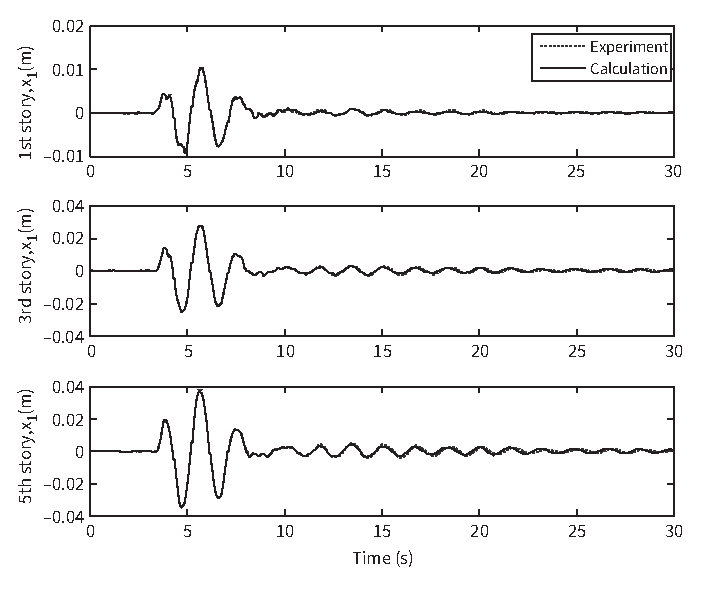
\includegraphics[width=0.8\textwidth] {figure/8-10b.eps}
   \label{fig:8-10b}
}
\caption{Comparison between calculated and experimentally measured responses under Northridge earthquake excitation.}
\label{fig:8-10}
\end{figure}

\begin{figure}[H]
\centering
\subfigure[force-displacement relation]{
   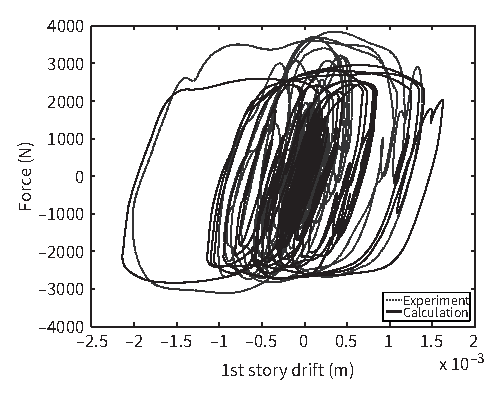
\includegraphics[width=0.45\textwidth] {figure/8-11a.eps}
   \label{fig:8-11a}
}
\subfigure[force-velocity relation]{
   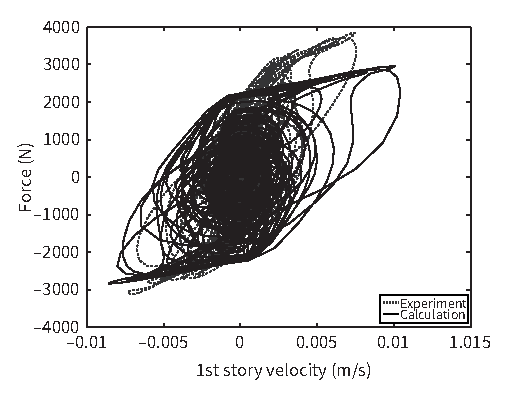
\includegraphics[width=0.45\textwidth] {figure/8-11b.eps}
   \label{fig:8-11b}
}
\caption{Comparison between calculated and experimentally measured hysteresis under El Centro earthquake excitation.}
\label{fig:8-11}
\end{figure}

\begin{figure}[H]
\centering
\subfigure[force-displacement relation]{
   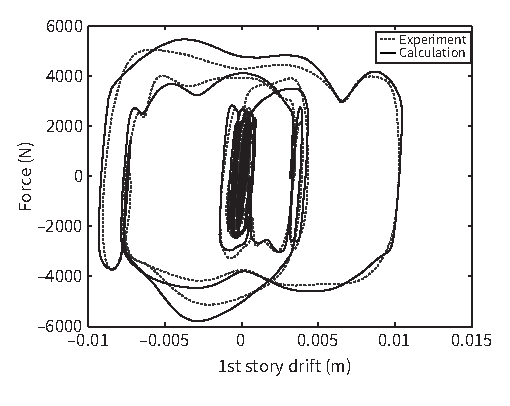
\includegraphics[width=0.45\textwidth] {figure/8-12a.eps}
   \label{fig:8-12a}
}
\subfigure[force-velocity relation]{
   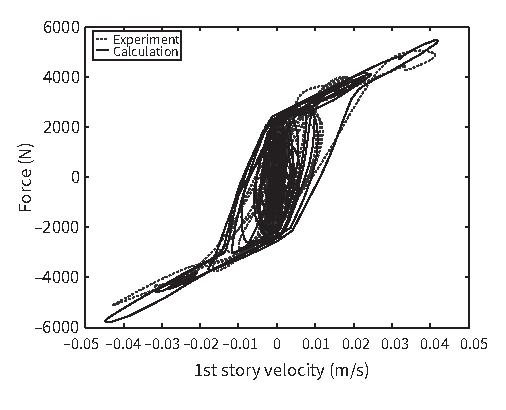
\includegraphics[width=0.45\textwidth] {figure/8-12b.eps}
   \label{fig:8-12b}
}
\caption{Comparison between calculated and experimentally measured hysteresis under Northridge earthquake excitation.}
\label{fig:8-12}
\end{figure}

\subsection{Applied Semi-active Control Algorithms}
\subsubsection{OPTIMIZATION OF BOUC-WEN PARAMETER BY INPUT CURRENTS}

In order to compare the results of the numerical analysis with the results of the semi-active hybrid testing method, the identification of the Bouc-Wen parameter corresponding to input currents is required. In this study, a sinewave excitation test is implemented, and Bouc-Wen parameters ($\alpha$, $A$, $c_{MR}$) are identified.

Figure~\ref{fig:8-13} shows a comparison between the test model and the identified Bouc-Wen model with respect to different input currents. The optimal parameter of the Bouc-Wen model is established by force-velocity and force-displacement relationships, as shown in Figure~\ref{fig:8-13a} and \ref{fig:8-13b}. For implementing the semi-active control of an MR damper, three parameters which are assumed to be polynomial, exponential functions of the input current are identified using the least square method. Figures~\ref{fig:8-13c}-\ref{fig:8-13e} show the results of each parameter identified and tested.

\begin{figure}[H]
\centering
\subfigure[force-displacement relation]{
   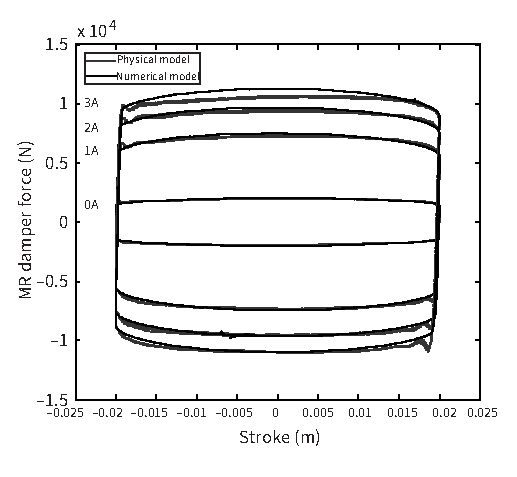
\includegraphics[width=0.45\textwidth] {figure/8-13a.eps}
   \label{fig:8-13a}
}
\subfigure[force-velocity relation]{
   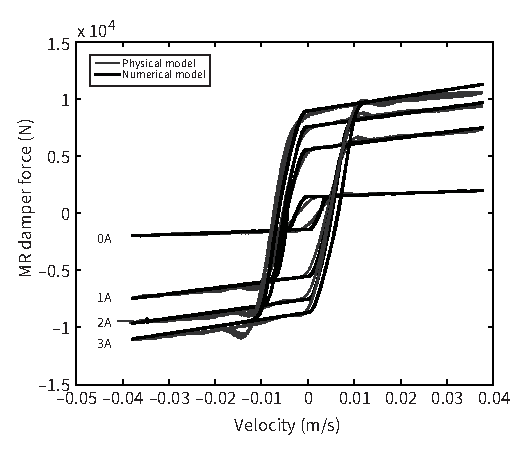
\includegraphics[width=0.45\textwidth] {figure/8-13b.eps}
   \label{fig:8-13b}
}
\subfigure[shape parameter]{
   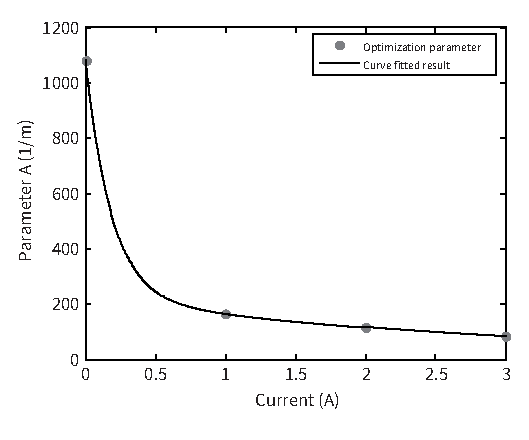
\includegraphics[width=0.3\textwidth] {figure/8-13c.eps}
   \label{fig:8-13c}
}
\subfigure[damping coefficient of an MR damper]{
   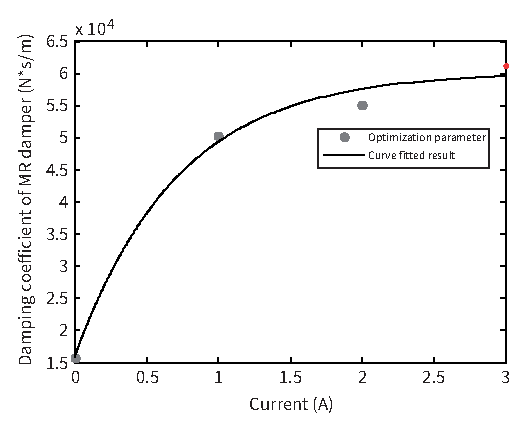
\includegraphics[width=0.3\textwidth] {figure/8-13d.eps}
   \label{fig:8-13d}
}
\subfigure[shape parameter $\alpha$]{
   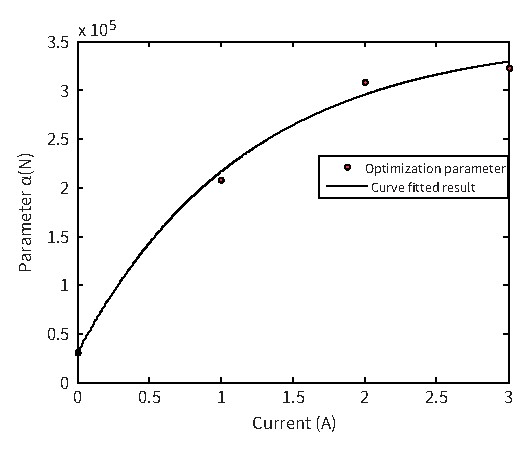
\includegraphics[width=0.3\textwidth] {figure/8-13e.eps}
   \label{fig:8-13e}
}
\caption{Identified Bouc-Wen parameters and the numerical model of an MR damper.}
\label{fig:8-13}
\end{figure}


\begin{align}
\alpha&=-324576.03\exp(-0.85x) + 354777.40 \label{eq:8-17} \\
c_{MR}&=-44567.17\exp(-1.4x) + 60330.96 \label{eq:8-18}\\
A&=854.7\exp(-5.476x) + 222.5\exp(-0.3321x) \label{eq:8-19}
\end{align}

where, $x$ is input current ($A$)

\subsubsection{Clipped-optimal Control Algorithm}
In terms of implementation, this control strategy seems to be the most direct because it can take advantage of the significant number of experimental and practical studies that have been conducted on active control strategies. The clipped-optimal algorithm that has been shown to be effective for use with the MR damper has been proposed by \citet{dyke1996modeling}. The clipped-optimal control approach involves designing a linear optimal controller $\matr{K}_{c}(s)$ that calculates a vector of desired control forces $\matr{f}_{c} = \left\{f_{c_{1}}, f_{c_{2}},...,f_{c_{n}}\right\}^{\top}$ based on the measured structural responses $\matr{y}$ and the measured control force vector $\matr{f}$ applied to the structure, that is,

\begin{equation}\label{eq:8-20}
\matr{f}_{c} = \mathcal{L}^{-1}\left\{-\matr{K}_{c}(s)\mathcal{L}\left\{\matr{y},\matr{f}\right\}^{\top}\right\}
\end{equation}

where, $\mathcal{L}\left\{\cdot\right\}$ is the Laplace transform.

Because the force generated in the MR damper is dependent on the local responses of the structural system, the desired optimal control force $f_{c_{i}}$ cannot always be produced by the MR damper. Only the control voltage $v_{i}$ can be directly controlled to increase or decrease the force produced by the device. Thus, a force feedback loop is incorporated to induce the MR damper to approximately generate the desired optimal control force $f_{c_{i}}$.

To induce the MR damper to approximately generate the corresponding desired optimal control force $f_{c_{i}}$, the command signal $v_{i}$ is selected as follows. When the $i-$th MR damper is providing the desired optimal force, the voltage applied to the damper should remain at the present level. If the magnitude of the force produced by the damper is smaller than the magnitude of the desired optimal force and the two forces have the same sign, the voltage applied to the current driver is increased to the maximum level so that the force produced by the damper is increased to match the desired control force. Otherwise, the commanded voltage is set to zero. The algorithm for selecting the command signal for the $i-$th MR damper is stated as Eq.~\eqref{eq:8-21}\citep{jansen2000semiactive}.

\begin{equation}\label{eq:8-21}
v_{i} = V_{\text{max}}H\left(\left\{f_{c_{i}}-f_{i}\right\}f_{i}\right)
\end{equation}

Although a variety of approaches may be used to design the optimal controller, linear quadratic regulator (LQR) methods are advocated because of their successful application. The optimal gain of a state vector based on the target building model with MR damper is used as follows:

\begin{align*}
\matr{K}_{c} = [&-98301479.1,110902868.9,\\
&-36659599.6,24569454,5, -12841877.0,\\
&-4926535.9, -3813412.5, -331115.5,\\
&-1239172.8, -1309155.8]
\end{align*}

For implementing the hybrid testing method experiment, the integrated MATLAB \textit{Simulink} controller is designed as shown in Figure~\ref{fig:8-14}. In the field testing application of this control law, it is required that a full structural state vector is obtained using a filter estimation method such as Observer/Kalman. However, because the hybrid testing method uses the structural model as a numerical model, this method has the advantage that the structural state variable is easily used in the experiment.

\begin{figure}[H]
\centering
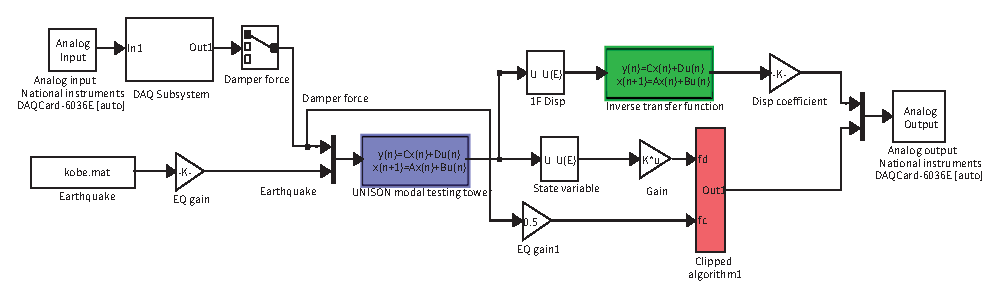
\includegraphics[width=1\textwidth] {figure/8-14.eps}
\caption{Clipped-optimal and hybrid testing method integrated controller.}
\label{fig:8-14}
\end{figure}

\subsubsection{MODULATED HOMOGENEOUS FRICTION ALGORITHM (MHF)}

This control strategy is originally developed for a variable-friction damper. In this approach, at every occurrence of local extremes in the deformation of the device, the normal force applied to the frictional interface is updated to a new value. At each local minimum or maximum in the deformation, the normal force $N_{i}(t)$ is chosen to be proportional to the absolute value of the semi-active damper deformation. The control law is written as Eq.~\eqref{eq:8-22}\citep{inaudi1997modulated}:

\begin{equation}\label{eq:8-22}
N_{i}(t)=g_{i}|P\left[\Delta_{i}(t)\right]|
\end{equation}

where $g_{i}$ is a positive gain and the operator $P\left[\cdot\right]$ as the prior-local-peak operator is defined as $P\left[\Delta_{i}(t)\right] = \Delta_{i}(t-s)$, where $s=\left\{\text{min }x\geq 0: \dot{\Delta}\left(t-x\right)=0\right\}$, defining $\Delta\left(t-s\right)$ as the most recent local extreme in the deformation.
Because this algorithm was developed for variable friction devices, the following modifications are needed when applying it to MR dampers.

\begin{enumerate}[(i)]
\item There is often no need to check if the force is greater than the static friction because MR dampers have no static friction.
\item A force feedback loop is used to induce the MR damper to produce approximately the frictional force corresponding to the required normal force.
\end{enumerate}
Thus, the goal is to generate a required control force with a magnitude of:

\begin{equation}\label{eq:8-23}
f_{n_{i}}=\mu g_{i}|P\left[\Delta_{i}(t)\right]=g_{n_{i}}|P\left[\Delta_{i}(t)\right]
\end{equation}

where the proportionality constant $g_{n_{i}}$ has a unit of stiffness N/mm.

As with the clipped-optimal control law, because the force produced by the MR damper cannot be directly commanded, a force feedback loop is used. The measured force is compared to the desired force determined by Eq.~\eqref{eq:8-23}, and the resulting control law is:

\begin{equation}\label{eq:8-24}
v_{i} = V_{\text{max}}H\left(f_{n_{i}}-|f_{i}|\right)
\end{equation}

where $V_{\max}$ is the maximum current value that can be offered for the MR damper.

An appropriate choice of $g_{n_{i}}$ will maintain the force $f_{n_{i}}$ within the operating envelope of each MR damper for the majority of the time, allowing the MR damper forces to approximate the desired force of each device closely. However, the optimal value of $g_{n_{i}}$ is dependent on the amplitude of the ground acceleration. In this study, the $g_{n_{i}}$ value is chosen as 150 kN/m based on the excitation of three earthquakes.

In addition, note that this control law is quite straightforward to implement because it only requires the measurement of the applied force and the relative displacements of the control device.

For applying the hybrid testing method experiment, the integrated MATLAB \textit{Simulink} controller is designed as shown in Figure~\ref{fig:8-15}.

\begin{figure}[H]
\centering
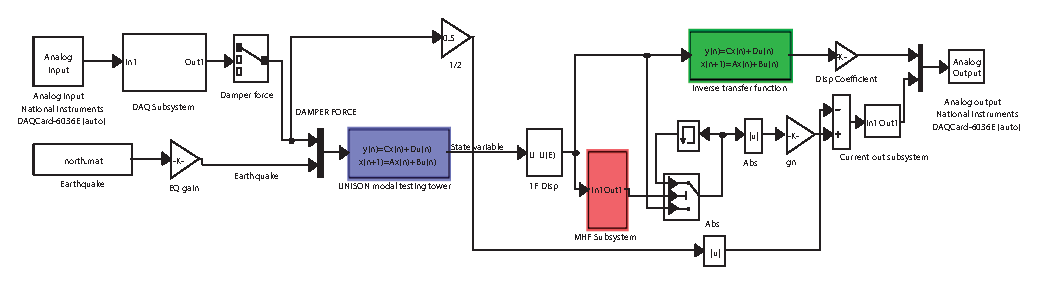
\includegraphics[width=1\textwidth] {figure/8-15.eps}
\caption{MHF and hybrid testing method integrated controller.}
\label{fig:8-15}
\end{figure}

\section{Testing Result}
\subsection{Passive Control Performance}

The hybrid testing method illustrated in Figure~\ref{fig:8-7} is implemented to evaluate the seismic performance of the passive-controlled MR damper used in this study. Except for the variation of the applied current to the MR damper (in the same manner as that above), four earthquake records are also given as the ground accelerations in Figure~\ref{fig:8-7}. The tests for the controlled case are carried out by increasing the current applied to the MR damper from 0 to 3 A. As shown in Figure~\ref{fig:8-8}, the test for the uncontrolled case is performed by removing the feedback loop of the control force generated by an MR damper into the control computer. Therefore, the numerical substructure is excited only by the ground input acceleration (even though a current of 0A was applied to the MR damper).

Figures~\ref{fig:8-16} and \ref{fig:8-17} show comparisons for the selected floors of the time histories of experimentally measured structural displacement responses to the excitation of two earthquake excitations, as the current applied to the MR damper is varied. Significant control effects are observed between the uncontrolled and the passive-off case but are not observed in the other passive-on cases with the increase of the applied current.

\begin{figure}[H]
\centering
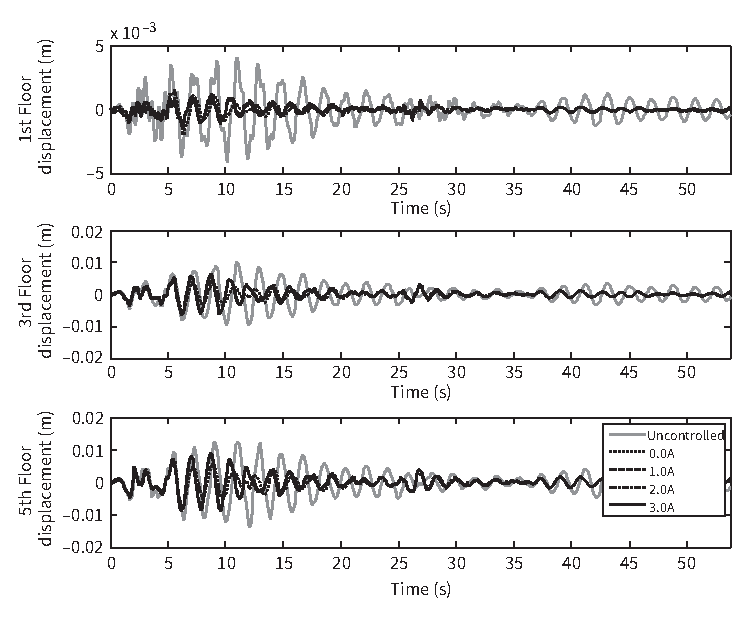
\includegraphics[width=1\textwidth] {figure/8-16.eps}
\caption{Experimental results, in the time domain under El Centro earthquake excitation at different applied currents.}
\label{fig:8-16}
\end{figure}

\begin{figure}[H]
\centering
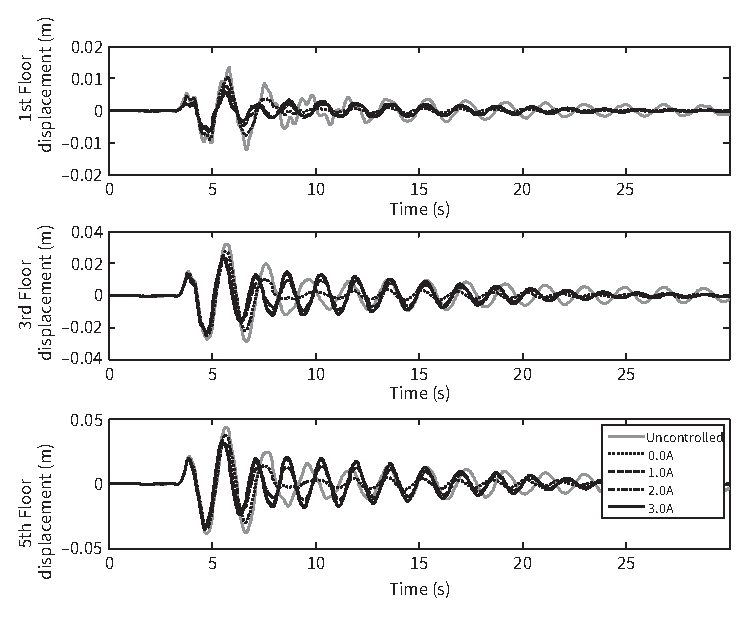
\includegraphics[width=1\textwidth] {figure/8-17.eps}
\caption{Experimental results, in the time domain under Northridge earthquake excitation at different applied currents.}
\label{fig:8-17}
\end{figure}

In addition, the displacement responses in the frequency domain to four earthquake excitations at different applied currents are compared to the first floors, as shown in Figure~\ref{fig:8-18}. The figures show that the peak in the uncontrolled case appears at 0.52 Hz, corresponding to the fundamental frequency of the numerical substructure under consideration, but the peak is shifted to the vicinity of 0.62 Hz as the applied current increases. This small amount of frequency shifting is due to the stiffening effect of the MR damper used in this study as the applied current is increased.

\begin{figure}[H]
\centering
\subfigure[El Centro earthquake]{
   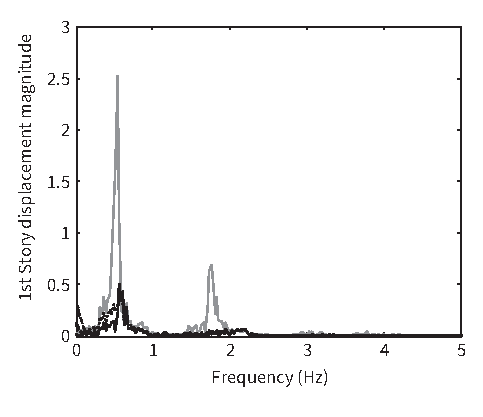
\includegraphics[width=0.45\textwidth] {figure/8-18a.eps}
   \label{fig:8-18a}
}
\subfigure[Kobe earthquake]{
   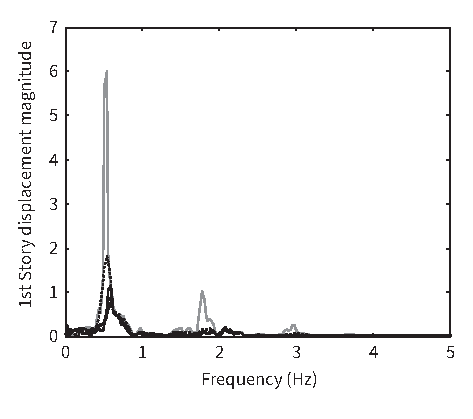
\includegraphics[width=0.45\textwidth] {figure/8-18b.eps}
   \label{fig:8-18b}
}
\subfigure[Northridge earthquake]{
   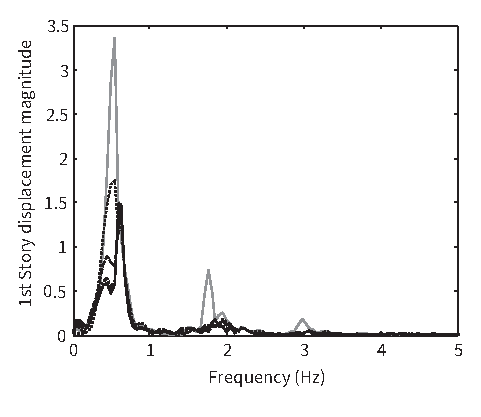
\includegraphics[width=0.45\textwidth] {figure/8-18c.eps}
   \label{fig:8-18c}
}
\subfigure[Hachinohe]{
   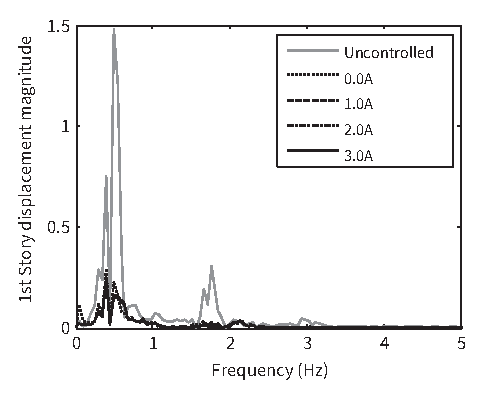
\includegraphics[width=0.45\textwidth] {figure/8-18d.eps}
   \label{fig:8-18d}
}
\caption{First-story displacements in the frequency domain at different applied currents.}
\label{fig:8-18}
\end{figure}

\subsection{Semi-active Control Performance}
Figure~\ref{fig:8-19} shows a comparison between numerical and experimental results for the clipped-optimal control under El Centro earthquake excitation based on identified Bouc-Wen parameters. As shown in Figure~\ref{fig:8-19}, the experimental and numerical results show different currencies. Moreover, because the peak responses are very important in evaluating seismic performance, it is critical to have large differences between the experimental and numerical results. These results are due to the nonlinearity of MR dampers which varies in the numerical model corresponding to frequencies of the piston and nonlinear reaction velocity of input currents. Consequently, these results prove that using the hybrid testing method is more practical in non-linear damper models such as MR dampers.

\begin{figure}[H]
\centering
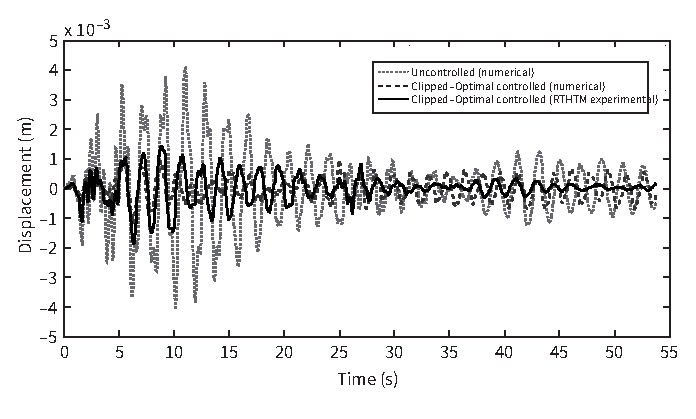
\includegraphics[width=1\textwidth] {figure/8-19.eps}
\caption{Comparison of numerical and experimental results under El Centro earthquake excitation.}
\label{fig:8-19}
\end{figure}

Figure~\ref{fig:8-20} shows a comparison between the first-floor displacements for the time histories of experimentally measured structural displacement responses to the excitation of three earthquake excitations, as the current applied to the MR damper is varied corresponding to each semi-active control algorithm. Significant control effects are observed between the uncontrolled and the passive control cases but are not observed in each semi-active control case of El Centro, as shown in Figure~\ref{fig:8-20a}. In Figure~\ref{fig:8-20c}, the clipped optimal control algorithms show remarkable performances in controlling displacement response.

\begin{figure}[H]
\centering
\subfigure[El Centro earthquake]{
   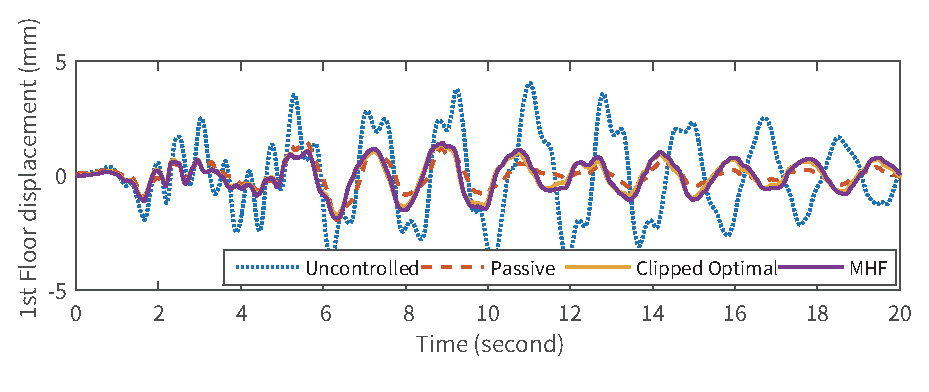
\includegraphics[width=0.8\textwidth] {figure/8-20a.eps}
   \label{fig:8-20a}
}
\subfigure[Kobe earthquake]{
   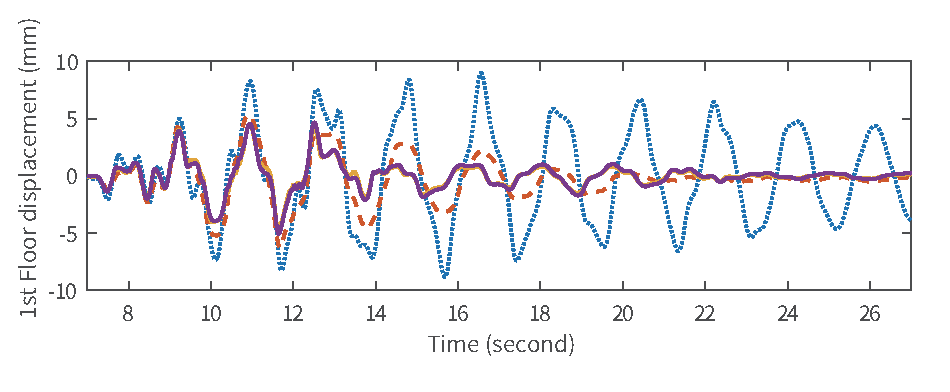
\includegraphics[width=0.8\textwidth] {figure/8-20b.eps}
   \label{fig:8-20b}
}
\subfigure[Northridge earthquake]{
   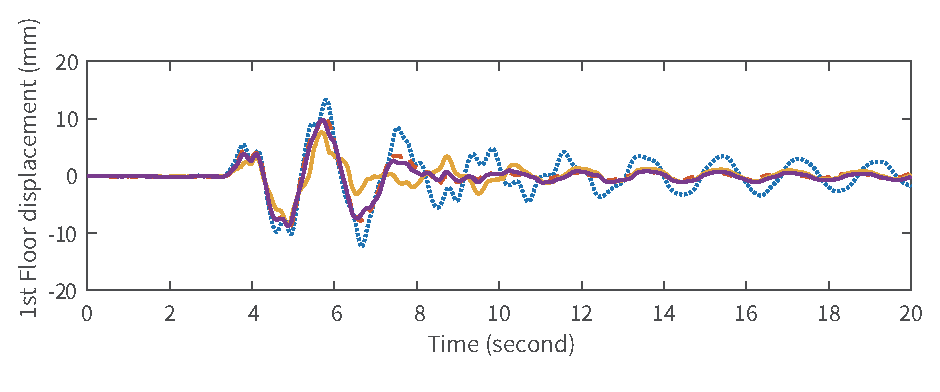
\includegraphics[width=0.8\textwidth] {figure/8-20c.eps}
   \label{fig:8-20c}
}
\caption{Passive and semi-active hybrid testing method experimental results(time domain).}
\label{fig:8-20}
\end{figure}

Also, the displacement responses in the frequency domain to three earthquake excitations applied to uncontrolled, passive, and semi-active controlled hybrid testing method are compared to the first floor, as shown in Figure~\ref{fig:8-21}. The figures show that an overall best control performance is achieved when the clipped optimal control algorithms are applied to the structure. However, all the results show insignificant control performance against the passive control. These results are influenced by the long-period model structure having 0.52 Hz and a scaled-down excitation load due to the UTM capacity. For the passive result, the peak response is shifted to the vicinity of 0.62 Hz in a semi-active controlled result. This small amount of frequency shifting is due to the stiffening effect of the MR damper used in this study as the applied current is increased for the passive control results.

\begin{figure}[H]
\subfigure[El Centro earthquake]{
   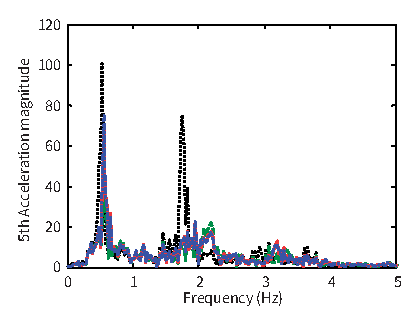
\includegraphics[width=0.45\textwidth] {figure/8-21a.eps}
   \label{fig:8-21a}
}
\hfill\subfigure[Kobe earthquake]{
   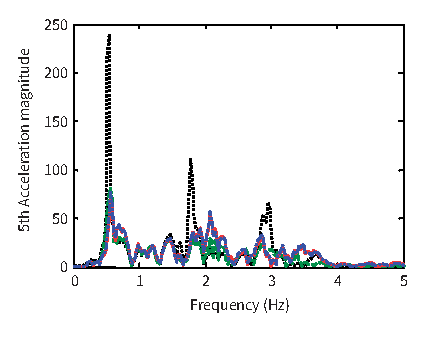
\includegraphics[width=0.45\textwidth] {figure/8-21b.eps}
   \label{fig:8-21b}
}
\subfigure[Northridge earthquake]{
   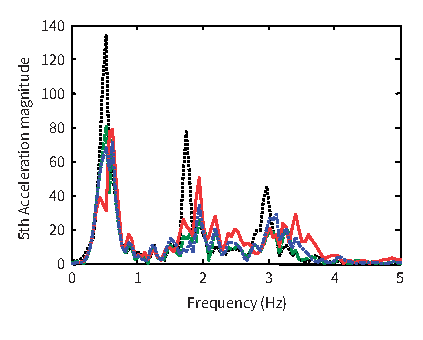
\includegraphics[width=0.45\textwidth] {figure/8-21c.eps}
   \label{fig:8-21c}
}
\hfill\subfigure{
   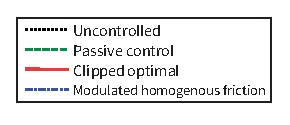
\includegraphics[width=0.25\textwidth] {figure/8-21d.eps}
}
\caption{Passive and semi-active hybrid testing method experimental results(frequency domain).}
\label{fig:8-21}
\end{figure}

\section{Summary}
In this chapter, the investigation of the hysteretic behavior of an MR damper and the seismic performance evaluation of a building structure, installed with an MR damper, are experimentally implemented using the hybrid testing method. In the tests, the building model that is identified from the force-vibration test results of a full-scale five-story building is adopted as a numerical substructure in this study. Also, an MR damper that corresponds to an experimental substructure is physically tested using a UTM. The Bouc-Wen model is used to calculate the control force of the MR damper used in this study, and its parameters are identified based on the experimental results from the hybrid testing method, which used a sinusoidal wave as the ground input acceleration. The hybrid testing method is validated because the hybrid testing results from the sinusoidal and earthquake excitations and the corresponding analytical results agreed well with each other. In particular, the hybrid testing method is highly reliable with the impulse-like seismic excitation such as that of the Northridge earthquake. In order to compare the results obtained from the hybrid testing method and the numerical analysis, Bouc-Wen model parameters are identified by each input current. The results of this comparison show that the hybrid testing method is more practical than the numerical analysis due to the non-linear variations of the reaction velocity and excitation frequency. The experimental results from the hybrid testing method for the passive control show that structural responses did not decrease further by the excessive control force, but they decreased with the increase of the current applied to the MR damper. In addition, the semi-active controlled result shows an insignificant control performance compared to the passively controlled result. It seems that the passive control forces of the MR damper already reached the optimal friction force by the proportional shear force of the first floor.